\documentclass[margin=10pt]{standalone}
\usepackage{cmbright}
%\renewcommand{\familydefault}{\sfdefault}
%
\usepackage{tikz}
\usetikzlibrary{arrows}
\usetikzlibrary{arrows.meta}
\usetikzlibrary{backgrounds}
\usetikzlibrary{decorations.markings}
\usetikzlibrary{fit}
\usetikzlibrary{matrix}
\usetikzlibrary{positioning}
\usetikzlibrary{shadows}

\begin{document}
{
\normalsize
%\large

\newsavebox\mybox
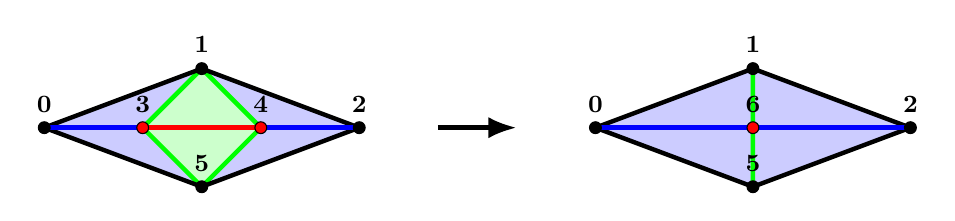
\begin{tikzpicture}[
		every node/.style = {
			draw,
			fill = white!5,
			align = center,
		},
		labeltxt/.style = {
			draw = none,
			fill = none,
			anchor = east,
			minimum width = 1.65cm,
			outer sep = 0,
			inner sep = 0,
		},
		every label/.append style = {
			text=black,
			font={\small\bfseries},
		},
		line/.style = {
			ultra thick,
		},
		point/.style = {
			fill=black,
			inner sep = 0pt,
			outer sep = 0pt,
			%minimum size = 1.5mm,
			% circle,
		},
		npoint/.style = {
			inner sep = 0pt,
			outer sep = 0pt,
			minimum size = 1.5mm,
			circle,
		},
		bgbox/.style = {
			densely dotted,
			rounded corners,
			fill = black!10,
			%drop shadow,
		},
		arr/.style = {
        	-Latex,
        },
        fabv/.style = {
        	fill = green!20,
        },
        fblw/.style = {
        	fill = red!20,
        },
        fnby/.style = {
        	fill = blue!20,
        },
 		]

	%\draw[step=1cm,black!80,very thin] (0,0) grid (15,8);
	%\draw[step=0.5cm,black!20,very thin] (0,0) grid (15,8);


	%% BEFORE
	\coordinate (3) at (1.75cm, 5cm);
	\coordinate (4) at (3.25cm, 5cm);
	\coordinate	(1) at (2.5cm, 5.75cm);
	\coordinate (5) at (2.5cm, 4.25cm);
	\coordinate (0) at (0.5cm, 5cm);
	\coordinate (2) at (4.5cm, 5cm);

	\fill[fnby] (0) -- (1) -- (2) -- (5) -- cycle;
	\fill[fabv] (1) -- (4) -- (5) -- (3) -- cycle;


	\draw[line, draw=red] (3) -- (4);
	\draw[line, draw=green] (3) -- (1) -- (4) -- (5) -- cycle;
	\draw[line, draw=black] (0) -- (1) -- (2) -- (5) -- cycle;
	\draw[line, draw=blue] (0) -- (3) (2) -- (4);

	\coordinate[npoint, label={3}, fill=red] (3) at (1.75cm, 5cm);
	\coordinate[npoint, label={4}, fill=red] (4) at (3.25cm, 5cm);
	\coordinate[npoint, label={1}, fill=black]	(1) at (2.5cm, 5.75cm);
	\coordinate[npoint, label={5}, fill=black] (5) at (2.5cm, 4.25cm);
	\coordinate[npoint, label={0}, fill=black] (0) at (0.5cm, 5cm);
	\coordinate[npoint, label={2}, fill=black] (2) at (4.5cm, 5cm);


	% BEFORE HASSE
	% \filldraw[draw=none, fill=black!20] (0,2) -- (2,2) -- (1,3.5) -- (0,3.5) -- cycle;
	% \filldraw[draw=none, fill=black!20] (5,2) -- (3,2) -- (4,3.5) -- (5,3.5) -- cycle;

	% \filldraw[line, densely dotted, fill=blue!20] (2,2) -- (1,3.5) -- (2,3.5) -- (2.5,2.75) -- cycle;
	% \filldraw[line, densely dotted, fill=blue!20] (3,2) -- (4,3.5) -- (3,3.5) -- (2.5,2.75) -- cycle;

	% \filldraw[line, fill=red!50] (2,2) -- (2.5,2.75) -- (3,2) -- cycle;
	% \filldraw[line, fill=green!30] (2,3.5) -- (2.5,2.75) -- (3,3.5) -- cycle;

	% \node[point] (a1) at (0cm,2cm) {};
	% \node[point] (b1) at (2cm,2cm) {};
	% \node[point] (c1) at (3cm,2cm) {};
	% \node[point] (d1) at (5cm,2cm) {};
	% \draw[line] (a1) -- (b1) -- (c1) -- (d1);

	% \node[point] (a2) at (0cm,3.5cm) {};
	% \node[point] (b2) at (2cm,3.5cm) {};
	% \node[point] (c2) at (3cm,3.5cm) {};
	% \node[point] (d2) at (5cm,3.5cm) {};
	% \draw[line] (a2) -- (b2) -- (c2) -- (d2);

	% \node[npoint,
	% 	  fill = red,
	% 	  label={[name=sl]east:{s}}
	% 	 ]
	% 	(s) at (2.5cm, 2.75cm) {};


	% \draw[line,arr] (5.5cm,2.75cm) -- (6.5cm, 2.75cm);
	\draw[line,arr] (5.5cm,5cm) -- (6.5cm, 5cm);


	%% AFTER
	\coordinate (6) at (9.5, 5cm);
	\coordinate	(1) at (9.5cm, 5.75cm);
	\coordinate (5) at (9.5cm, 4.25cm);
	\coordinate (0) at (7.5cm, 5cm);
	\coordinate (2) at (11.5cm, 5cm);

	\fill[fnby] (0) -- (1) -- (2) -- (5) -- cycle;

	\draw[line] (0) -- (5) -- (2) -- (1) -- cycle;
	\draw[line, draw=green] (1) -- (6) -- (5);
	\draw[line, draw=blue] (0) -- (6) -- (2);

	\coordinate[npoint, label={6}, fill=red] (6) at (9.5,5cm);
	\coordinate[npoint, label={1}, fill=black] (1) at (9.5cm, 5.75cm);
	\coordinate[npoint, label={5}, fill=black] (5) at (9.5cm, 4.25cm);
	\coordinate[npoint, label={0}, fill=black] (0) at (7.5cm, 5cm);
	\coordinate[npoint, label={2}, fill=black] (2) at (11.5cm, 5cm);


	% \filldraw[draw=none, fill=black!20] (7,2) -- (9.5,2) -- (8.25,3.5) -- (7,3.5) -- cycle;
	% \filldraw[draw=none, fill=black!20] (12,2) -- (9.5,2) -- (10.75,3.5) -- (12,3.5) -- cycle;
	% \filldraw[line, densely dotted, fill=blue!20] (9.5cm,2cm) arc (-45:0:1) -- (9.5cm, 2.7cm) -- (9.5cm, 3.5cm) -- (10.75cm, 3.5cm) -- cycle;
	% \filldraw[line, densely dotted, fill=blue!20] (9.5cm,2cm) arc
	%  (-135:-180:1) -- (9.5cm, 2.7cm) -- (9.5cm, 3.5cm) -- (8.25cm, 3.5cm) -- cycle;


	% \filldraw[line, fill=green!30] (9.5cm, 2cm) arc(-45:0:1) -- (9.20cm, 2.707cm) arc(-180:-135:1);

	% \node[point] (aa1) at (7cm,2cm) {};
	% \node[point] (bb1) at (9cm,2cm) {};
	% \node[point] (cc1) at (10cm,2cm) {};
	% \node[point] (dd1) at (12cm,2cm) {};
	% \draw[line] (aa1) -- (bb1) -- (cc1) -- (dd1);

	% \node[point] (aa2) at (7cm,3.5cm) {};
	% \node[point] (bb2) at (9cm,3.5cm) {};
	% \node[point] (cc2) at (10cm,3.5cm) {};
	% \node[point] (dd2) at (12cm,3.5cm) {};
	% \draw[line] (aa2) -- (bb2) -- (cc2) -- (dd2);

	% \node[npoint,
	% 	  fill = red,
	%  	  label={[name=sl]south:{s}}
	%  	 ]
	% 	(ss) at (9.5cm, 2cm) {};

\end{tikzpicture}
}% end size


\end{document}